\section{Von der Recherche zum Feinkonzept}
Um Eckpfeiler für die zu Beginn des Projekts benötigten Recherchen zu erhalten, musste das Problem grob in seine Teilprobleme zerlegt werden. Aus dieser Zerlegung resultierten die Bereiche Kommunikation zwischen elektronischen Geräten, Möglichkeiten zur Objekterkennung und Objektverfolgung, diverse Flugobjekte und Fahrantriebe, Bedarf von Dreh- und Wurfmechanismen sowie ein Versorgungskonzept. \\
Um Übersicht über die Teilprobleme zu behalten wurde eine Funktionsskizze geschaffen, welche in  Abbildung \ref{fig:Funktionsskizze} ersichtlich ist.\\
\begin{figure}[h!]
	\centering
	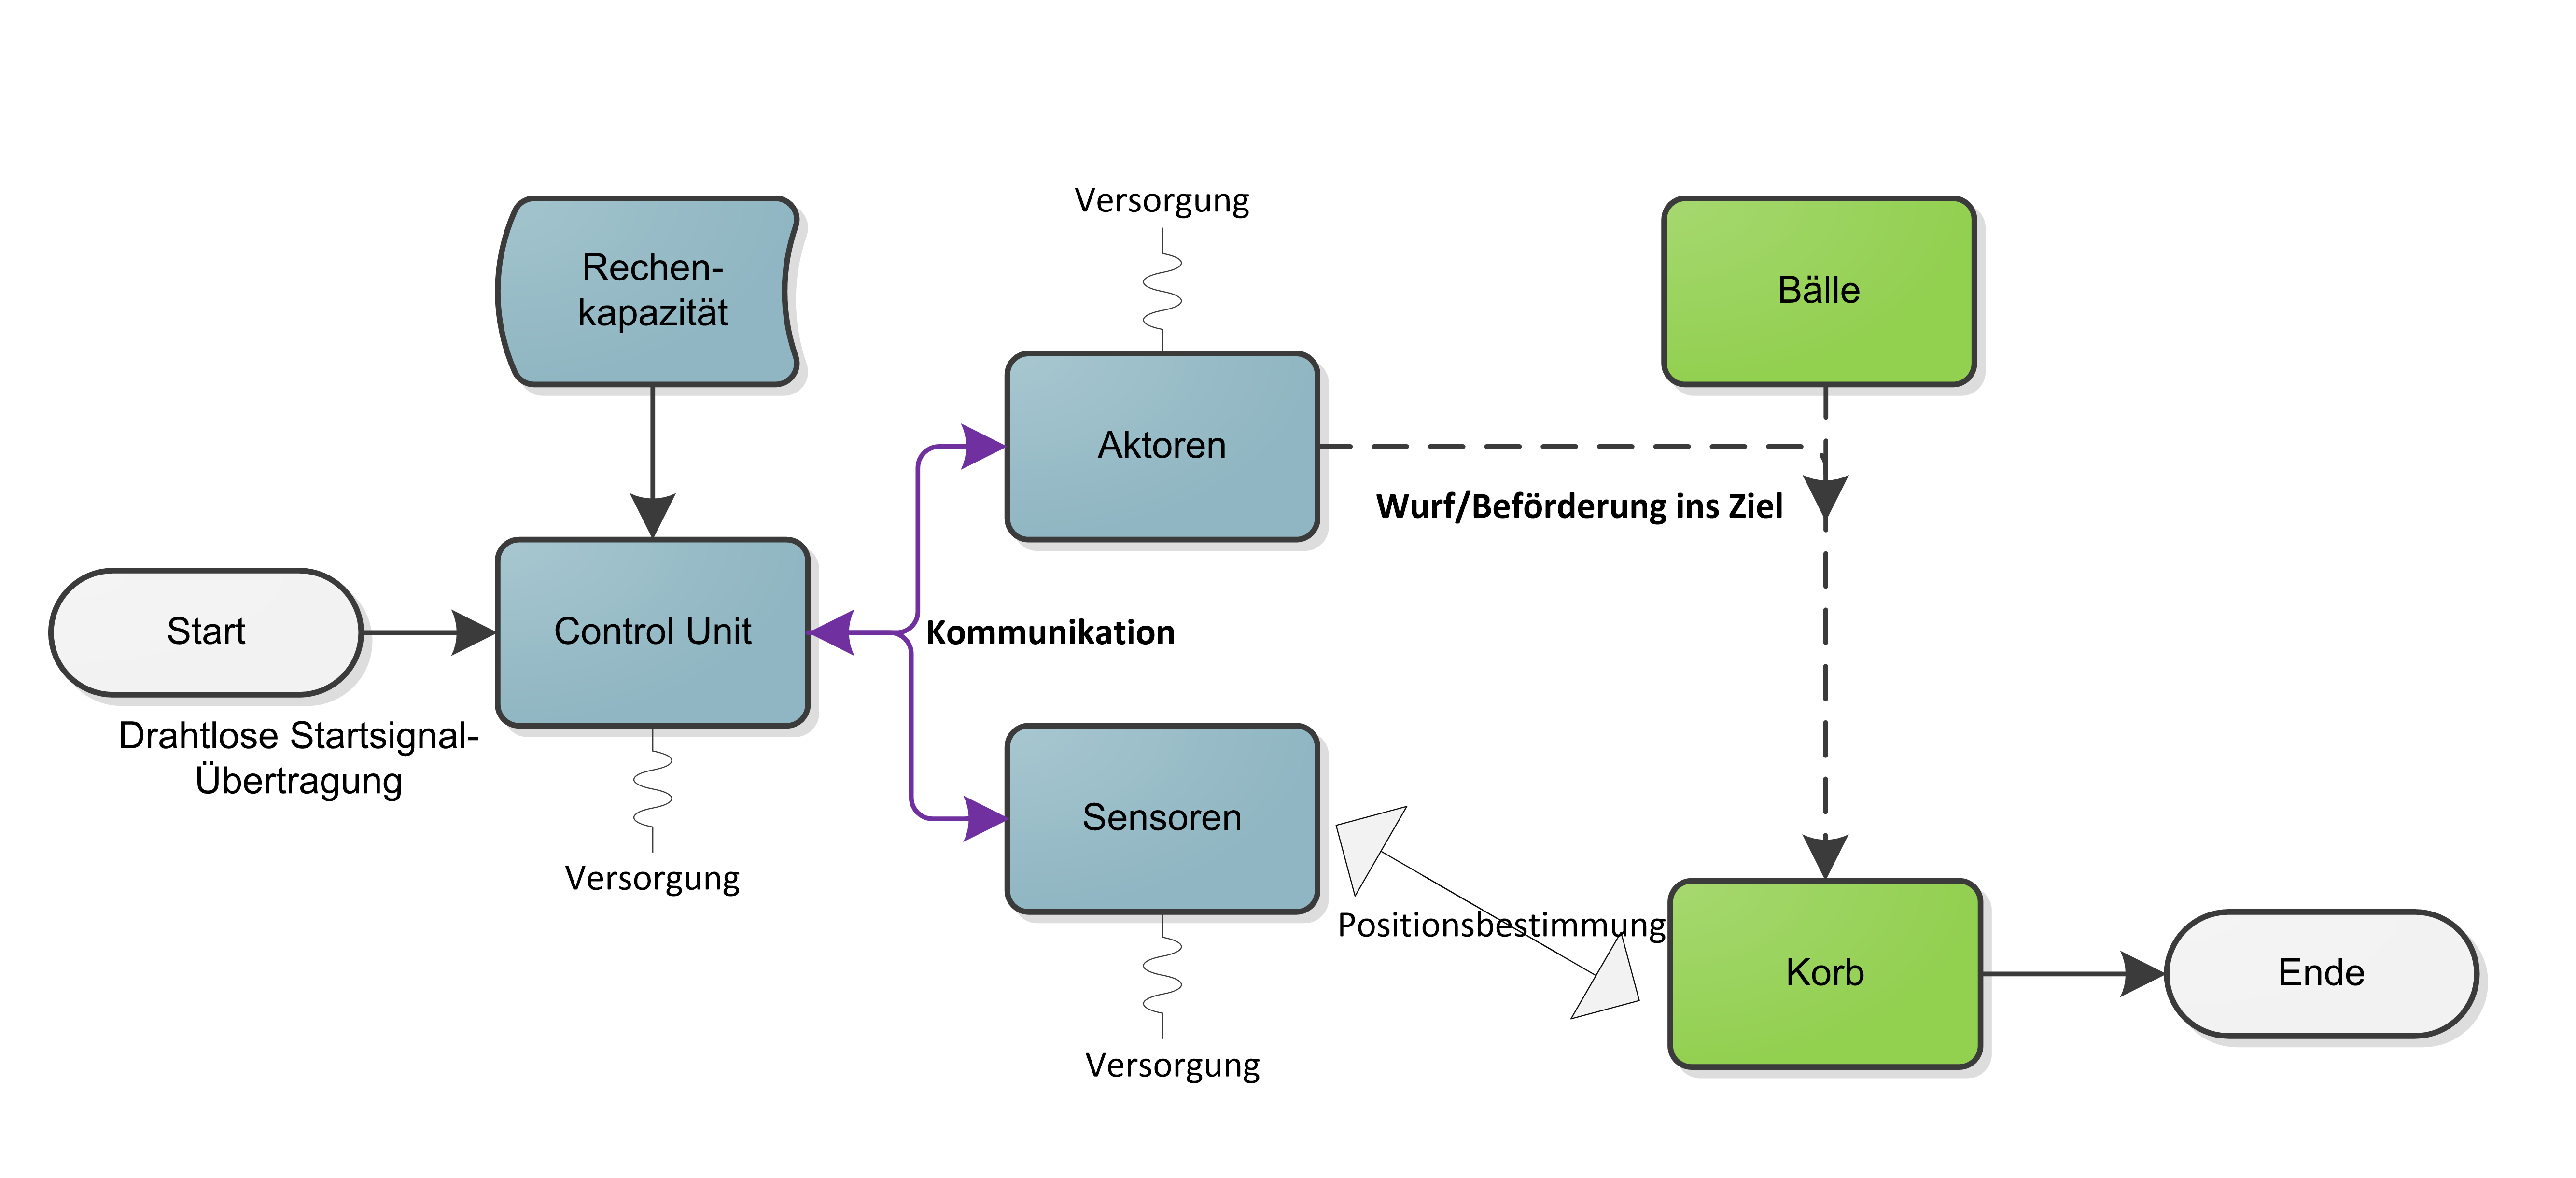
\includegraphics[width=1\textwidth]{Enddokumentation/Varianten/Bilder/Funktionsskizze.png}
	\caption{Funktionsskizze}
	\label{fig:Funktionsskizze}
\end{figure}
\\\\
Nach der Ermittlung dieser Teilprobleme mussten für die einzelnen Bereiche nach Lösungsansätzen recherchiert werden. Die Resultate dieser Recherche, sowie die danach folgende Bewertung der gefundenen Lösungen ist aus Platzgründen im Anhang hinterlegt. Um die Ergebnisse der Bewertung sinnvoll als Entscheidungshilfe einsetzen zu können, wurden sie kompakt zu einem Grobkonzept zusammengefasst.\\
\\
Jedes Teilproblem ist bezüglich den Vor- und Nachteilen nach den definierten Zielsetzungen bewertet worden. Dadurch lassen sich grafisch geeignete Kombinationsmöglichkeiten herleiten und untereinander vergleichen. Um möglichst vielen differenzierten Ansätzen Rechnung zu tragen, wurden vier Varianten während einer Diskussionsrunde festgelegt.\\
\\
\newpage
\begin{figure}[h!]
	\centering
	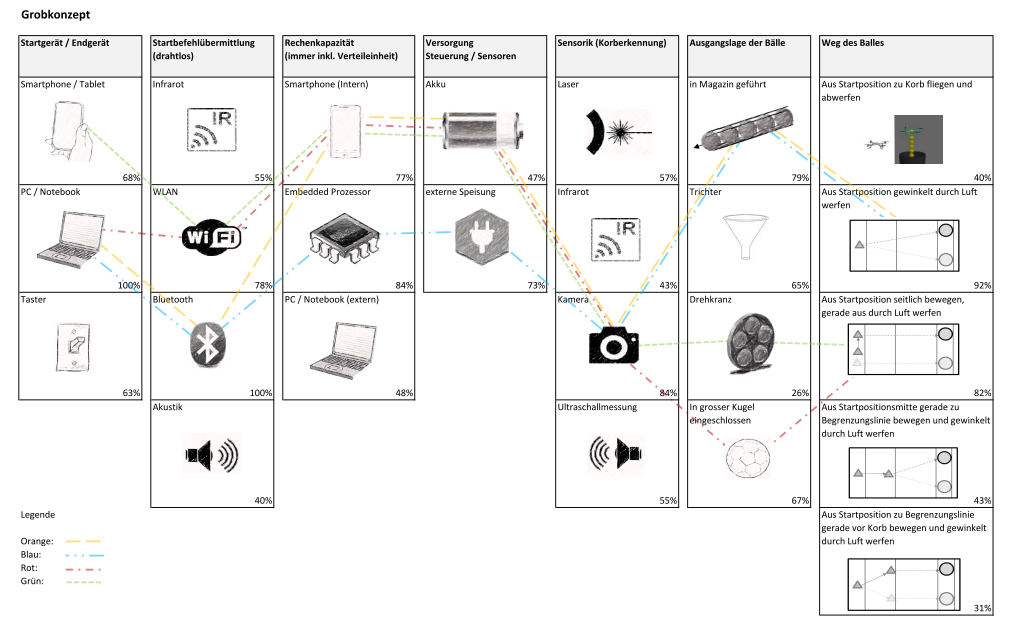
\includegraphics[width=1.08\textwidth]{Enddokumentation/Varianten/Bilder/Grobkonzept.png}
	\caption{Lösungsansätze für die einzelnen Teilprobleme mit den vier gewählten Varianten}
	\label{fig:Grobkonzept}
\end{figure}
Die blaue Variante ist die Kombination aller Lösungsansätze mit der höchsten Prozentzahl. Die rote Variante basiert auf der Idee, die Bälle in eine Kugel einzuschliessen, das Gerät parallel zur Spielfeldwand zu verschieben und den Korb mit einer Smartphone-Kamera zu erkennen. Der Ballwerfer soll durch einen Akkumulator mit Energie versorgt werden. Als Ausgangslage führt die grüne Variante die Bälle in einem Drehkranz und befördert diese einzeln in den Korb, die restlichen Kriterien werden kongruent zur zweiten Variante ausgeführt. Im orangen Konzept befördert der Ballwerfer die Bälle aus der Startposition in bogenförmiger Kurve in den Korb. Die Ausgabe der Bälle erfolgt vereinzelt. Die übrigen Teilprobleme verwenden wiederum, äquivalent zur zweiten Variante eine Smartphone-Kamera zur Korberkennung und einen Akkumulator als Energieversorgung.\\
\\\\
Die Entscheidung fiel auf die orange Variante. Diese bietet als gesamtes Konzept die erfolgversprechendste und effizienteste Lösung, bezüglich der Zielsetzung des Teams. \\

\begin{tabular}{p{1cm}p{10cm}}
	\multirow{3}{4cm}	{
\includegraphics[width=1cm]{Enddokumentation/Varianten/Bilder/info_icon.png}}
	 & Die detaillierte Beschreibung der Lösungsfindung (von der Funktionsskizze bis zum Feinkonzept) war Aufgabe des zweiten Testates und ist als Dokument im Anhang beigelegt. \\
\end{tabular}\\
\\
\\
Nach der Entscheidung für eine Variante folgt die weitere Ausarbeitung des Konzeptes
in einzelne Feinkonzepte. Die ursprünglich sieben Teilprobleme wurden in 19 Subteilprobleme
aufgesplittet. Zu jedem Subteilproblem existieren wiederum Lösungsvarianten. Im Unterschied zum Grobkonzept erfolgt die Bewertung nicht mit Prozenten, sondern werden die Lösungsvarianten miteinander verglichen und nach aktuellem Wissenstand eine oder eventuell auch mehrere Lösungsvarianten ausgewählt. 


